\begin{figure*}[!t]
  \centering
  \subfloat[The execution time of forward computation] {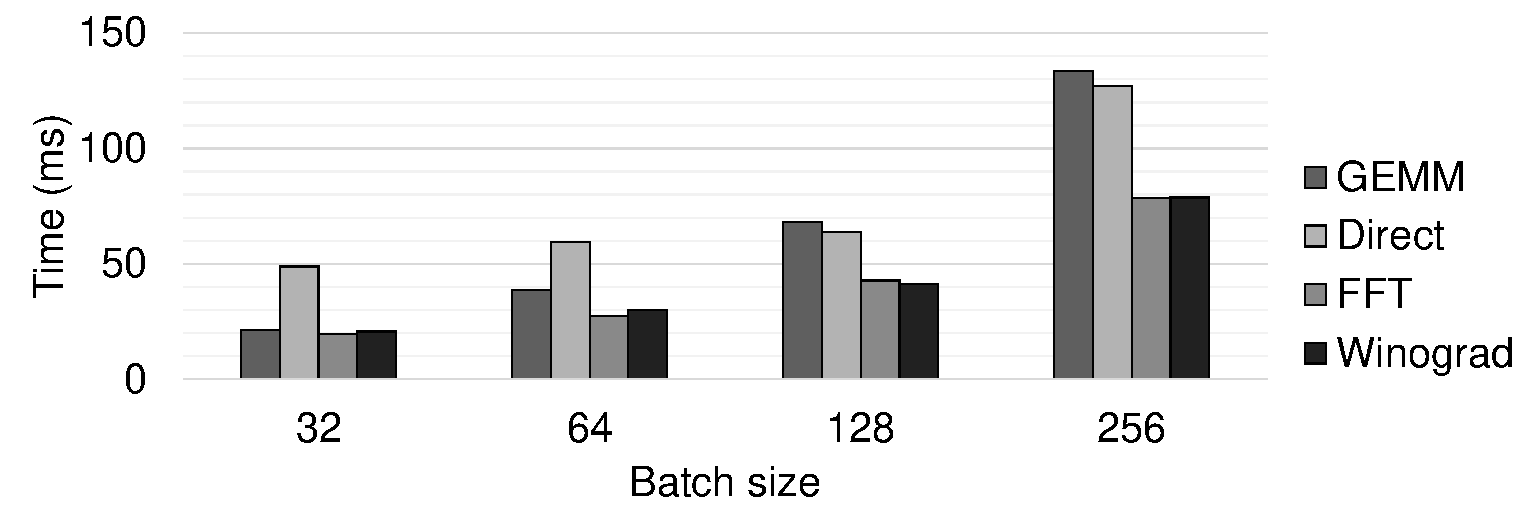
\includegraphics[width=.45\linewidth]{./figures/gpu_time_fwd}
  \label{fig_gpu_time_fwd}}
  \subfloat[The execution time of backward computation] {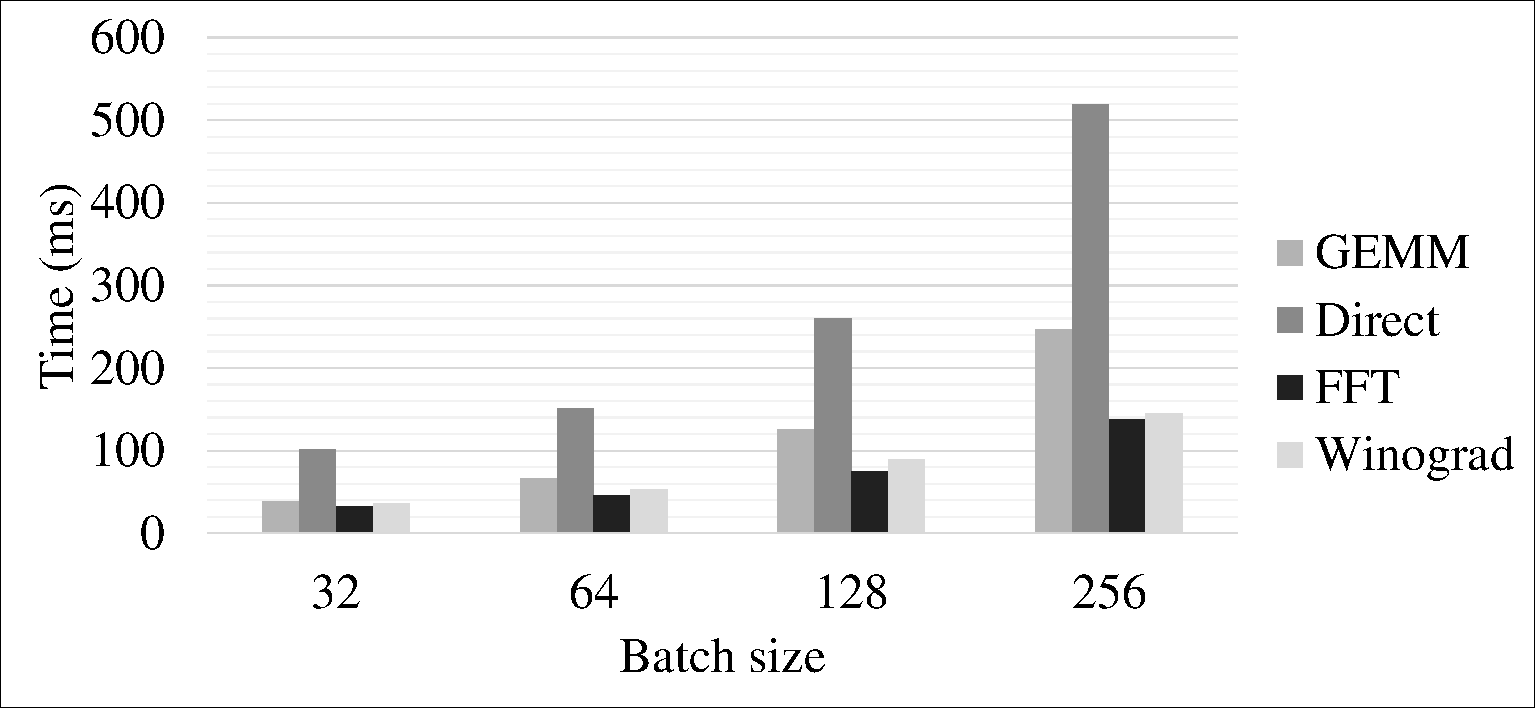
\includegraphics[width=.45\linewidth]{./figures/gpu_time_bwd}
  \label{fig_gpu_time_bwd}}
  \hfil
  \subfloat[The execution time of forward computation from \textsf{conv3} to \textsf{conv5}] {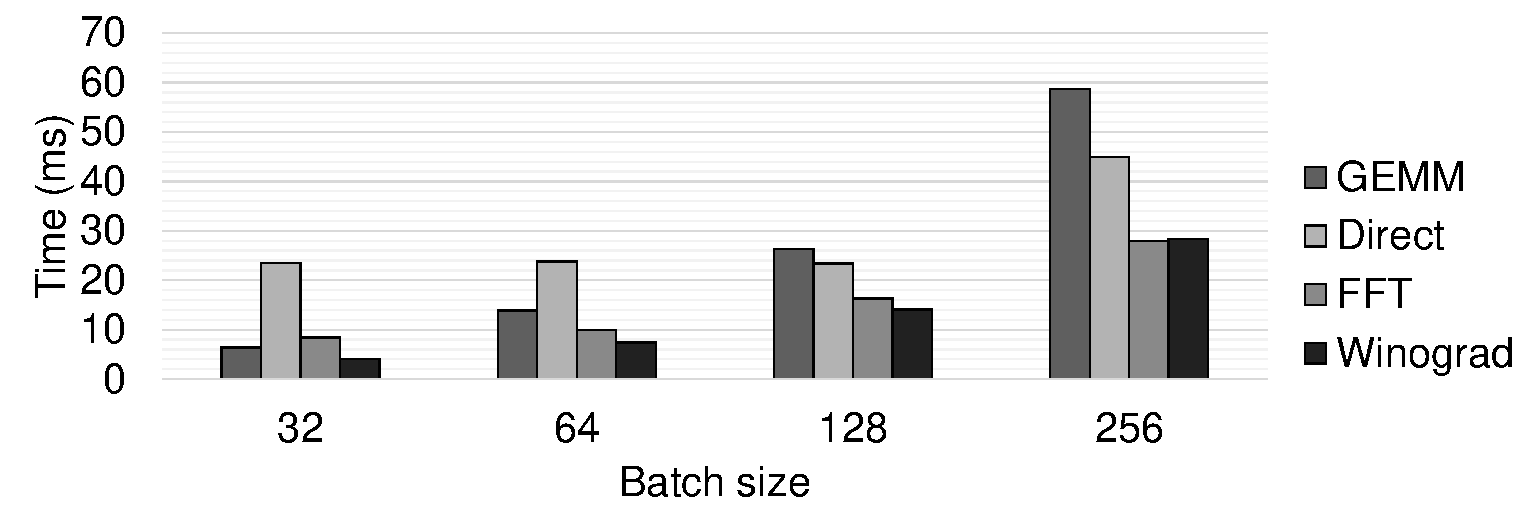
\includegraphics[width=.45\linewidth]{./figures/gpu_time_conv345}
  \label{fig_gpu_time_conv345}}
  \subfloat[Peak GPU memory usage] {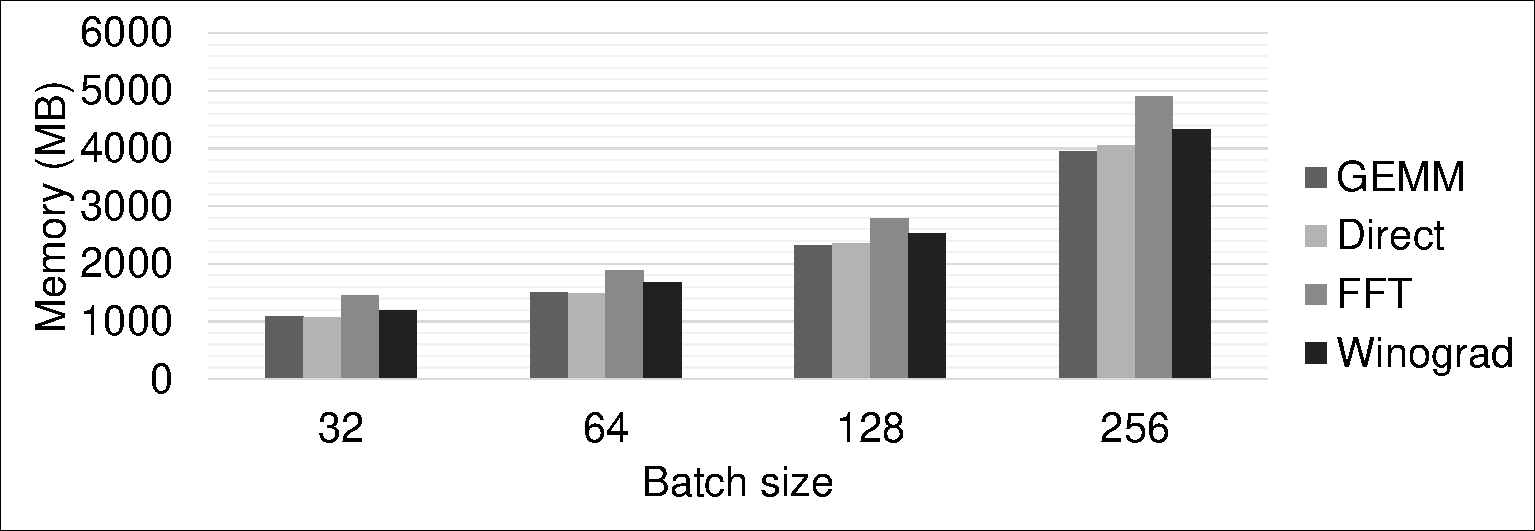
\includegraphics[width=.45\linewidth]{./figures/gpu_mem_kernels}
  \label{fig_gpu_mem}}
  \caption{Execution time and memory usage between different convolution algorithms in training.}
  \label{fig_conv_time}
\end{figure*}%

\section{Effect of Convolution Algorithms}
\label{convolution-algorithms}
In this section, we compare the performance of different convolution algorithms on a single GPU. These algorithms were introduced in Section~\ref{sec:algorithms}. 

\subsection{Backward and Forward convolution}
The backpropagation of a convolution layer requires 2 convolutions: backward data (\textsf{BD}) convolution and backward filter (\textsf{BW}) convolution. Backward data convolution generates gradient input to the previous layer while backward filter convolution computes gradients of the layer parameters. Backward convolution and forward convolution of a convolution layer are symmetric. Hence theoretically the backward computation time should be a double of the forward computation time. Since \textsf{BW} convolution has to write gradients for every parameter of the layer, it is more memory intensive than the others. \Comment{added a subsection for backward convolution}

\subsection{Execution Time}
Figure~\ref{fig_conv_time} shows execution time comparisons between GPU kernels of different convolution algorithms (\textsf{GEMM}, \textsf{Direct}, \textsf{FFT}, and \textsf{Winograd}) on a single GPU. We vary the batch size from 32 to 256. Since the convolution layers take most of the execution time in a CNN, using an efficient convolution algorithm in the CNN model is an important design decision. All comparisons are done with AlexNet built by Torch 7 because currently it is the only framework that officialy supports newest versions of cuDNN and Cuda-convnet3. Randomly generated images are used for the input to remove the I/O latency. The forward and backward computation times are measured and averaged for 100 iterations (\textit{i.e.}, batches). 

\textsf{Winograd} and \textsf{FFT} perform better than \textsf{Direct} or \textsf{GEMM} most of the time as shown in Figure~\ref{fig_conv_time} (a), (b), and (c). Since many recent CNN models use $3 \times 3$ kernel for convolution layers\cite{vgg}, the forward computation time of \textsf{conv3},  \textsf{conv4} and \textsf{conv5} is separately measured in Figure~\ref{fig_gpu_time_conv345}.

The total training time (the forward computation time + the backward computation time) of \textsf{FFT} is the best for all batch sizes. However, for $3 \times 3$ convolution kernels with small batch sizes, \textsf{Winograd} performs better than \textsf{FFT} while \textsf{FFT} scales better with large batch sizes. In addition, \textsf{Direct} (\textit{i.e.}, cuda-convnet) scales bad when the batch size is smaller than 128 while \textsf{GEMM} sclaes almost linearly.

Figure~\ref{fig_gpu_mem} shows peak GPU memory usage for each convolution algorithms. \textsf{FFT} occupies the most GPU memory, using about 20\% more memory than \textsf{GEMM}. 

\begin{figure}[htbp]
  \centering
  \subfloat[The execution time of the forward computation] {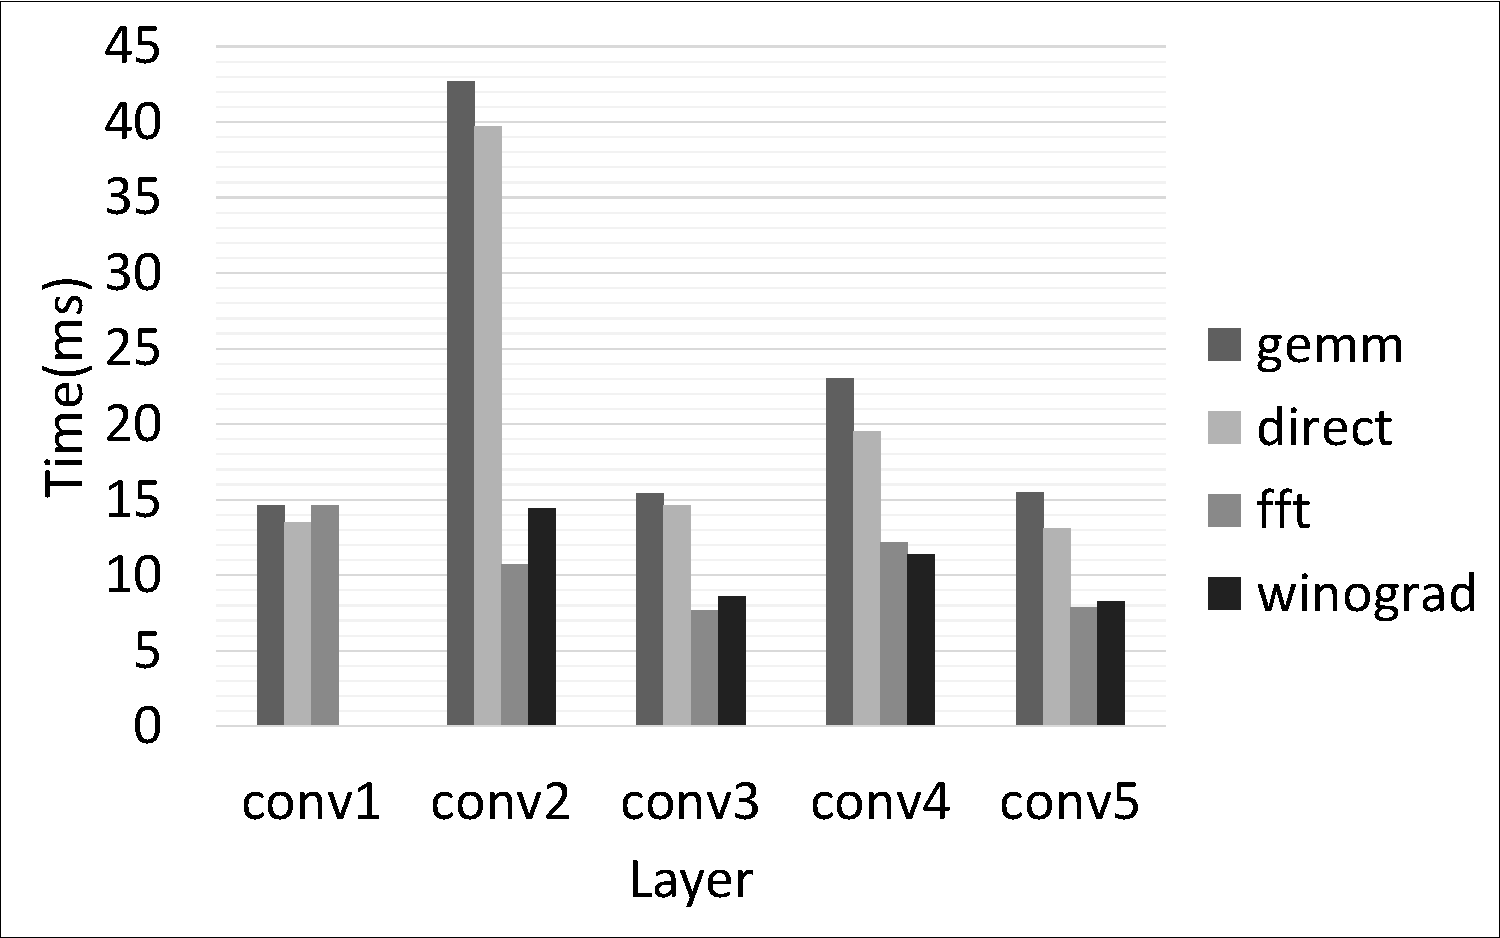
\includegraphics[width=.9\linewidth]{./figures/layerwise_fwd}
  \label{fig_layerwise_fwd}}

  \subfloat[The execution time of the backward computation] {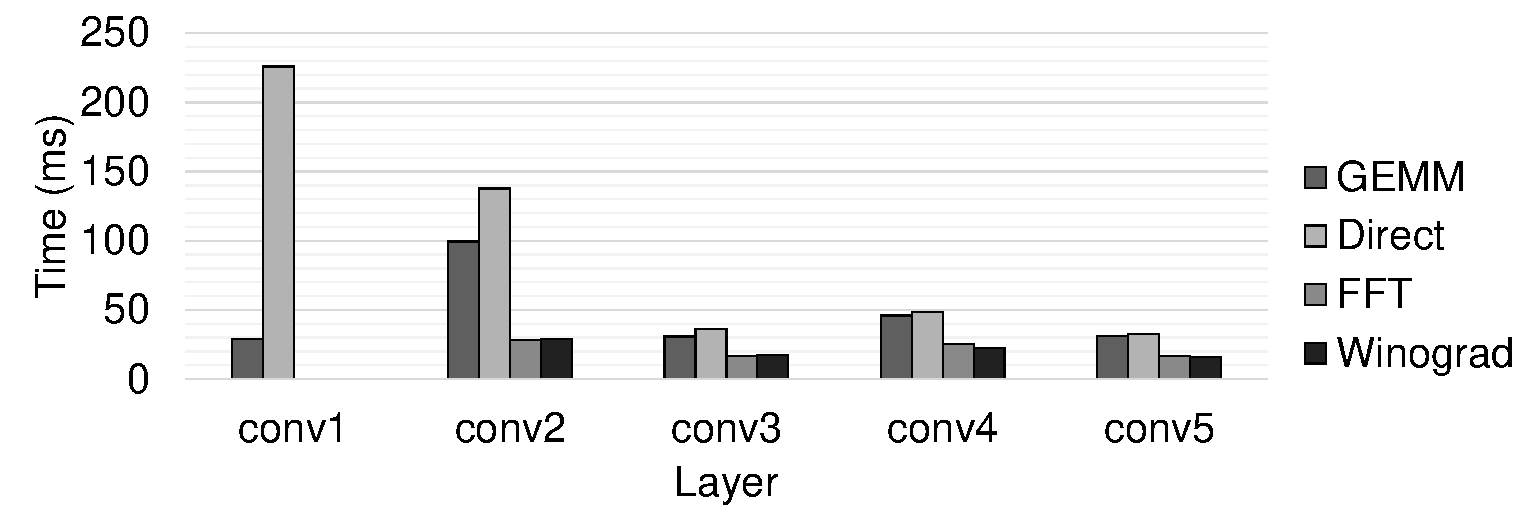
\includegraphics[width=.9\linewidth]{./figures/layerwise_bd}
  \label{fig_layerwise_bd}}

  \subfloat[FP operation count in the forward computation] {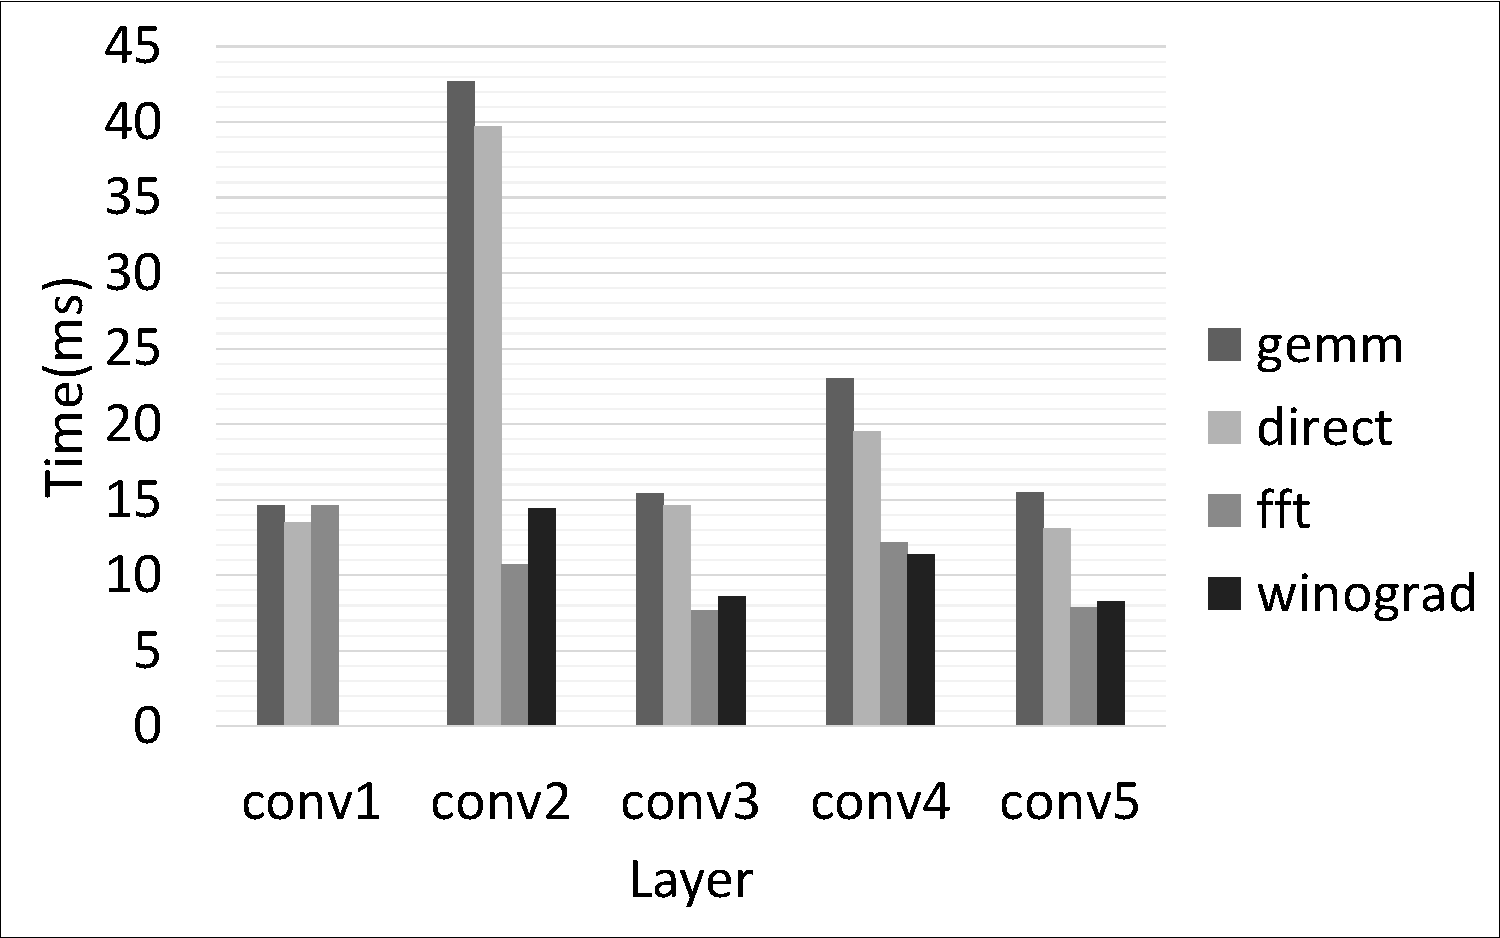
\includegraphics[width=.9\linewidth]{./figures/layerwise_fwd}
  \label{fig_layerwise_flop_count}}

  \subfloat[Compute-memory ratio of Backward filter convolution kernels] {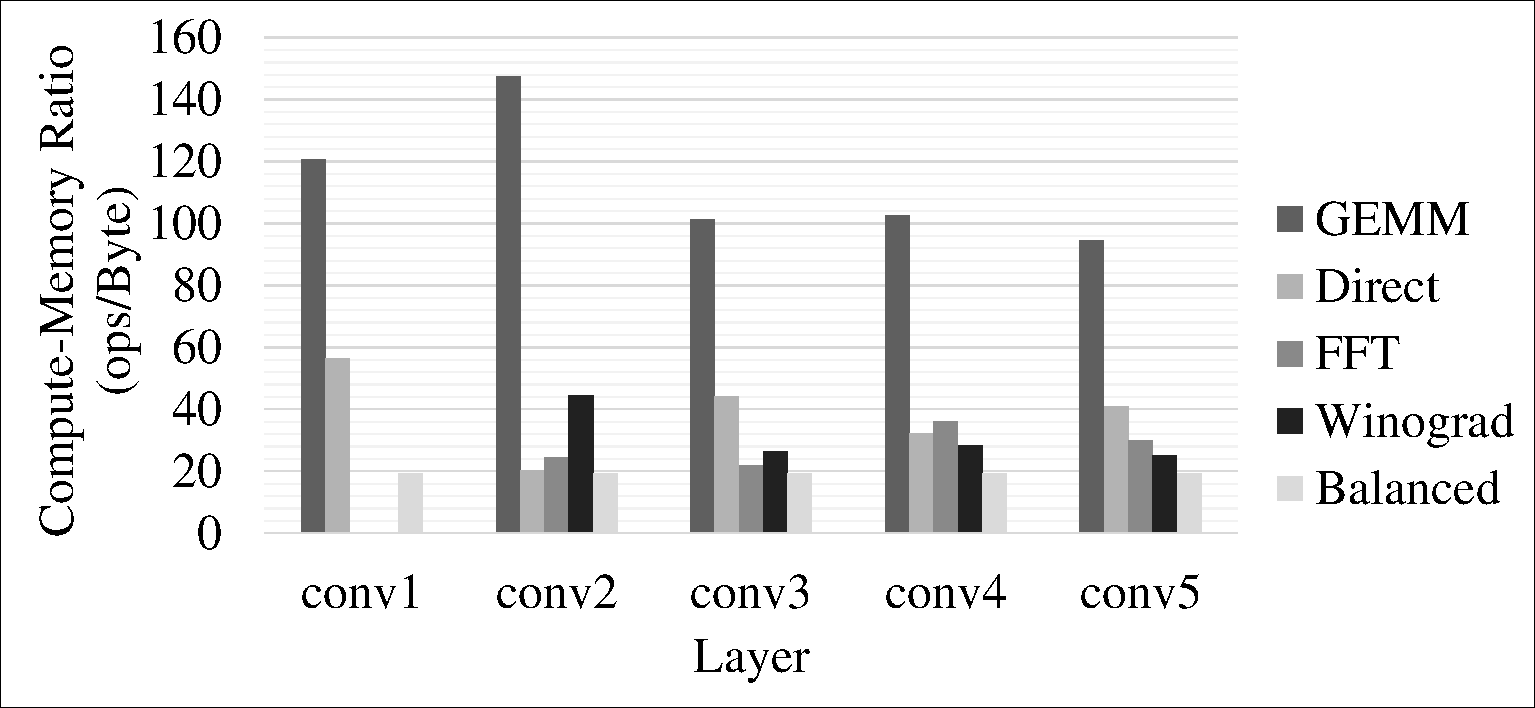
\includegraphics[width=.9\linewidth]{./figures/layerwise_mem_compute}
  \label{fig_layerwise_mem_compute}}%compute-memory ratio chart added

  \caption{Layerwise analysis of different convolution algorithms.}
  \label{fig_layerwise}
\end{figure}

\subsection{Layerwise Analysis}

Figure~\ref{fig_layerwise} shows layerwise analysis of different convolution algorithms on a single GPU. The batch size is set to 256, and the NVIDIA nvprof profiler is used to gather statistics.

As shown in Figure~\ref{fig_layerwise_bd}, the main performance limiter of \textsf{Direct} (\textit{i.e.},cuda-convnet) is the backward computation in \textsf{conv1} layer. The reason of the slowdown is low parallelism in GPU kernels of \textsf{Direct} that implement \textsf{conv1} layer. While NVIDIA Titan X has 3072 CUDA cores, the number of CUDA theads in the GPU kernels is only 1024. This make \textsf{Direct} slower than other algorithms in \textsf{conv1}. 

{\bf Floating-point operation count}. Figure~\ref{fig_layerwise_flop_count} compares floating-point (FP) operation counts of different convolution algorithms in the forward computation. The count is exactly the same in the backward computation kernels. The numbers are measured with the NVIDIA nvprof profiler. \textsf{Theoretical} stands for the theoretically computed count. The result tells us that \textsf{FFT} is usually the fastest because of much less FP operation count (\textit{i.e.}, much less algorithm complexity). Especially, \textsf{FFT} is much faster than others in \textsf{conv2} with $5 \times 5$ convolution filter because the complexity of the FFT algorithm does not depend on the filter size. \textsf{Winograd} also reduces FP operation count by more than half. Thus, its performance is comparable to \textsf{FFT} in the layers with $3 \times 3$ convolution filters (\textsf{conv3}, \textsf{conv4}, and \textsf{conv5}).

{\bf Compute-memory Ratio}. The theoretical maximum FP throughput of NVIDIA Titan X is 6 TFLOPS (floating-point operations per second), and maximum memory bandwidth is 336GB/s. Therefore balanced compute-memory ratio of Titan X is 18.3 FP operations per byte. Fig~\ref{fig_layerwise_mem_compute} shows compute-memory ratio of \textsf{BW} convolution kernels with the balanced ratio of Titan X. We divide FP operation counts to the device memory transaction bytes to calculate compute-memory ratio of the kernels. Since other convolution kernels are less memory intensive than \textsf{BW} convolution, the result indicates that convolution algorithms are compute intensive on a GPU rather than memory intensive. Therefore reduced algorithm complexity of \textsf{FFT} and \textsf{Winograd} result in faster convolutions. \Comment{//changed into compute-memory ratio}

\subsection{Summary}
We conducted layerwise kernel comparison of different convolution algorithms. The convolution kernels have high compute-memory ratio, indicating that they are compute intensive. \textsf{FFT} and \textsf{Winograd} perform significantly better than \textsf{GEMM} or \textsf{Direct} due to reduced algorithm complexity. \textsf{FFT} scales better on large batch and filter sizes while \textsf{Winograd} scales better on smaller batch and filter sizes. Carefully choosing a convolution kernel can make more than $4\times$ difference in a layer computation time. \Comment{//summary for analysis B updated}